\documentclass{beamer}

% Choose an aesthetic theme
\usetheme{Madrid}
% \usecolortheme{seagull} % Uncomment if you prefer to use the seagull color theme
\usefonttheme{serif}

% Packages for mathematical symbols and environments
\usepackage{amsmath, amssymb, amsthm}
\usepackage{colortbl} % For row coloring
% Packages for algorithms
\usepackage{algorithm}
\usepackage{algpseudocode} % Using algpseudocode for better flexibility

% Packages for figures
\usepackage{graphicx}
\usepackage{booktabs} % For better table formatting, if needed
\usepackage{caption}  % For customizing captions

% Title and Author Information
\title{Bandit-style Geometric decision algorithm against an Adaptive adversary}
\author{Amirreza Velaei}
\institute{Sharif University of Technology}
\date{\today}

\begin{document}

% Slide 1: Title Slide
\begin{frame}
    \titlepage
\end{frame}

% Slide 2: Outline
\begin{frame}{Outline}
    \tableofcontents
\end{frame}

% Section 1: Introduction and Background
\section{Introduction and Background}

\begin{frame}{Online Geometric Optimization in the Bandit Setting}
    \begin{itemize}
        \item
        \textbf{Paper Title}: Online Geometric Optimization in the Bandit 
        Setting Against an Adaptive Adversary \\
        \item \textbf{Authors :}  H. Brendan McMahan \& Avrim Blum
        \item \textbf{Published in:} 2004
        \item \textbf{Conference:} Learning Theory, Springer Berlin Heidelberg
    \end{itemize}

\end{frame}
\subsection{A Gentle Introduction to Online Optimization}
\begin{frame}{Introduction to Online Optimization}
    \textbf{Definition:} Online optimization involves making a sequence of decisions based on incoming data, where each decision is made without knowledge of future data. \\
    Two fundamental assumptions in online optimization:
    \begin{enumerate}
        \item \textbf{Bunded Losses:} The losses determined by an adversary should not be allowed to be unbounded.
        \item \textbf{Bounded Decision Set:}  The decision set must be somehow bounded and/or structured, though not necessarily finite.
    \end{enumerate}
\end{frame}

\subsection{Expert Advice}
\begin{frame}{Prediction from Expert Advice}
    \begin{itemize}
        \item \textbf{Prediction from Expert Advice} is a framework in online learning and decision-making.
        \item Involves making sequential predictions by aggregating advice from a set of experts.
        \item The goal is to perform nearly as well as the best expert in hindsight.
    \end{itemize}
\end{frame}

\begin{frame}{Key Components}
    \begin{enumerate}
        \item \textbf{Experts:} Sources that provide predictions or advice.
        \item \textbf{Learner (Main Character):} Aggregates expert advice to make decisions.
        \item \textbf{Feedback:} Information about the actual outcome to update future predictions.
        \item \textbf{Objective:} Minimize the difference between the learner's performance and the best expert's performance.
    \end{enumerate}
\end{frame}

\begin{frame}{Family Members as Experts}
    \begin{itemize}
        \item Main character decides whether to take an umbrella each day.
        \item Three family members act as \textbf{experts} providing daily weather predictions, the father, mother, and brother.
    \end{itemize}
    \begin{figure}
        \centering
        
\includegraphics[width=0.4\linewidth]{images/openart-image_7K5I2JtA_1735594988581_raw.jpg}
        \caption{Family Members as Experts}
    \end{figure}
\end{frame}

\begin{frame}{Example Scenario}
    \begin{table}[ht]
        \centering
        \caption{Daily Weather Predictions and Outcomes}
        \begin{tabular}{|c|c|c|c|c|}
            \hline
            \textbf{Day} & \textbf{Father} & \textbf{Mother} & \textbf{Brother} & \textbf{Actual Weather} \\
            \hline
            \only<1->{1 & \texttt{No Rain} & \texttt{No Rain} & \texttt{Rain} & \texttt{Rain} \\ \hline}
            \only<2->{2 & \texttt{Rain} & \texttt{No Rain} & \texttt{Rain} & \texttt{No Rain} \\ \hline}
            \only<3->{3 & \texttt{Rain} & \texttt{No Rain} & \texttt{No Rain} & \texttt{Rain} \\ \hline}
            \only<4->{4 & \texttt{No Rain} & \texttt{Rain} & \texttt{No Rain} & \texttt{No Rain} \\ \hline}
            \only<5->{5 & \texttt{Rain} & \texttt{No Rain} & \texttt{No Rain} & \texttt{Rain} \\ \hline}
            \only<6->{\textbf{Cost} & 2 & 4 & 3 & - \\ \hline}
        \end{tabular}
    \end{table}
\end{frame}

% Slide 1: Weighted Majority Algorithm
\begin{frame}{Weighted Majority Algorithm}
    \begin{itemize}
        \item \textbf{Mechanism:}
            \begin{itemize}
                \item Assigns a weight to each expert based on their past performance.
                \item Aggregates predictions by considering these weights.
                \item Updates weights multiplicatively based on the correctness of experts' predictions.
            \end{itemize}
        \item \textbf{Applications:}
            \begin{itemize}
                \item Ensemble learning in machine learning.
                \item Financial decision-making.
            \end{itemize}
    \end{itemize}
\end{frame}

% Slide 2: How Weighted Majority Works
\begin{frame}{How Weighted Majority Works}
    \textbf{Algorithm Steps:}
    \begin{enumerate}
        \item \textbf{Initialization:} Assign equal weights to all experts.
        \item \textbf{Prediction}
        \[
            \text{Prediction} = \text{sign}\left(\sum_{i=1}^{N} w_t(i) \cdot \text{Prediction}_t(i)\right)
        \]
        \item \textbf{Update Weights:} After observing the outcome, update weights:
        \[
            w_{t+1}(i) = 
            \begin{cases}
                w_t(i) & \text{if expert } i \text{ was correct} \\
                w_t(i) \cdot \varepsilon & \text{if expert } i \text{ was incorrect}
            \end{cases}
        \]
        \item \textbf{Iteration:} Repeat the prediction and update steps for each round.
    \end{enumerate}
    \textbf{Parameters:}
    \begin{itemize}
        \item $N$: Number of experts.
        \item $\varepsilon \in (0,1)$: Penalty factor for incorrect experts.
    \end{itemize}
\end{frame}

\begin{frame}{Regret Bound for Weighted Majority}
    \textbf{Lemma :} Denote by $M_t$ the number of mistakes the algorithm makes until time $t$, and by $M_t(i)$ the number of mistakes made by expert $i$ until time $t$. Then, for any expert $i \in [N]$ we have
        \begin{align*}
        M_T \leq 2(1+\varepsilon)M_T(i) + \frac{2\log N}{\varepsilon}
    \end{align*}
    \vspace{0.5 em}
    \textbf{Corollary :} The regret of the WM algorithm is bounded by
    \begin{align*}
        M_T \leq 2M_T(i^*) + O(\sqrt{M_T(i^*) log N})
    \end{align*} 
    where $i^*$ is the best expert.\\
    \vspace{0.5 em}
    \textbf{Proof:} Just let $\varepsilon^* = \sqrt{\frac{log N}{M_T(i^*)}}$.
\end{frame}

\begin{frame}{Regret Bound Proof}
    \textbf{Proof:}
    \begin{itemize}
        \item Let $\phi_t = \sum_{i=1}^{N} w_i(t)$. Note that $\phi_{1} = N$.
        \item If the prediction is wrong, then $\phi_{t+1} \leq \frac{1}{2} \phi_t(1-\varepsilon) + \frac{1}{2} \phi_t$.
        \item Thus $\phi_{t} \leq \phi_1 (1-\varepsilon)^{M_t} = N(1-\varepsilon)^{M_t}$.
        \item By definition, $w_T(i) = (1-\varepsilon)^{M_T(i)}$. Also $w_t(i) \leq \phi_t$.
        \item $(1-\varepsilon)^{M_T(i)} \leq N(1-\varepsilon)^{M_T} \rightarrow M_T(i) log(1-\varepsilon) \leq log N + M_T log(1-\varepsilon)$.
        \item Using the fact that $-x-x^2 \leq log(1-x) \leq -x$ for $x \in (0,1)$, we get:
        \begin{align*}
            -M_T(i) (\varepsilon + \varepsilon^2) \leq log N - M_T \frac{\varepsilon}{2} \rightarrow M_T \leq 2(1+\varepsilon)M_T(i) + \frac{2log N}{\varepsilon}
        \end{align*}
    \end{itemize}
\end{frame}


% Slide 3: Randomized Weighted Majority
\begin{frame}{Randomized Weighted Majority Algorithm}
    \begin{itemize}
        \item \textbf{Algorithm Steps:}
            \begin{enumerate}
                \item \textbf{Initialization:} Set $w_1(i) = 1$ for all experts.
                \item \textbf{Probability Assignment:}
                \[
                    P_t(i) = \frac{w_t(i)}{\sum_{j=1}^{N} w_t(j)}
                \]
                \item \textbf{Expert Selection:} Choose expert $i$ with probability $P_i(t)$.
                \item \textbf{Prediction and Update:} Make prediction based on selected expert and update weights as in Weighted Majority.
            \end{enumerate}
        \item \textbf{Better Regret Bound:} \\
        \begin{align*}
            \mathbb{E}[M_T] \leq (1+\varepsilon)M_T(i^*) + \frac{log N}{\varepsilon}
        \end{align*}
    \end{itemize}
\end{frame}

% Slide 4: Randomized Weighted Majority Proof
\begin{frame}{RWM Regret Bound Proof}
    \textbf{Proof:}
    Let $\phi_t = \sum_{i=1}^{N} w_i(t)$ and $\tilde{m}_t$ be an indicator variable for the event that the prediction is wrong at time $t$ and $\tilde{m}_t(i) = 1$ if expert $i$ is wrong at time $t$.
    \begin{itemize}
        \item Note that 
        \begin{align*}
            \phi_{t+1} = \sum_{i=1}^{N} w_i(t)(1-\varepsilon\tilde{m}_t(i)) &= \phi_t (1-\varepsilon\sum_{i=1}^{N} P_t(i)\tilde{m}_t(i)) \\
            &= \phi_t (1-\varepsilon \mathbb{E}[\tilde{m}_t]) \leq \phi_t e^{-\varepsilon \mathbb{E}[\tilde{m}_t]}
        \end{align*}
        \item With the same argument as in the WM proof, we get:
        \begin{align*}
            (1-\varepsilon)^{M_T(i)} &\leq N e^{-\varepsilon M_T}\\
            \rightarrow M_T(i) log(1-\varepsilon) &\leq log N - \varepsilon \mathbb{E}[M_T]\\
            \rightarrow - M_T (\varepsilon + \varepsilon^2) &\leq log N - \varepsilon \mathbb{E}[M_T]\\
            \rightarrow \mathbb{E}[M_T] &\leq (1+\varepsilon)M_T(i^*) + \frac{log N}{\varepsilon}
        \end{align*}
    \end{itemize}
\end{frame}

\subsection{Bandit Algorithms}
\begin{frame}{Introduction to Multi-Armed Bandit Algorithms}
    \begin{itemize}
        \item \textbf{Definition:} 
        A framework for making a sequence of decisions under uncertainty, aiming to maximize cumulative rewards.
        
        \item \textbf{Key Concepts:}
        \begin{itemize}
            \item \textbf{Exploration:} Trying different actions to gather more information.
            \item \textbf{Exploitation:} Selecting the best-known action to maximize immediate reward.
        \end{itemize}
        
        \item \textbf{Types of Bandit Problems:}
        \begin{itemize}
            \item \textbf{Stochastic Bandits:} Rewards are drawn from fixed probability distributions.
            \item \textbf{Contextual Bandits:} Incorporates contextual information to make more informed decisions.
        \end{itemize}
        
        \item \textbf{Applications:}
        \begin{itemize}
            \item Recommendation Systems
            \item Clinical Trials
            \item Online Advertising
        \end{itemize}
    \end{itemize}
\end{frame}

% Slide 2: Bandit Algorithms in Online Advertising
\begin{frame}{Bandit Algorithms in Online Advertising}
    \begin{itemize}
        \item \textbf{Use Case:} Optimizing Ad Selection to Maximize CTR
        
        \item \textbf{How It Works:}
        \begin{itemize}
            \item Each ad variant is considered an arm of the bandit.
            \item The algorithm dynamically selects which ad to display based on past performance.
            \item Balances exploration (trying new ads) with exploitation (showing top-performing ads).
        \end{itemize}
        
    \end{itemize}
    
    \vspace{0.5cm}
    \begin{figure}
        \centering
        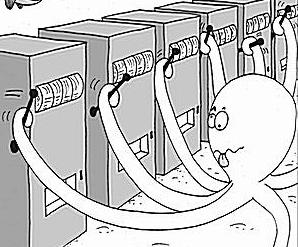
\includegraphics[width=0.4\linewidth]{images/bandit_setting.jpg}
        \caption{Bandit Setting}
    \end{figure}
\end{frame}


% Slide 3: Online Optimization and Bandit Algorithms
\begin{frame}{Online Optimization vs. Bandit Algorithms}
    Both online optimization and bandit algorithms involve sequential decisions, but differ in feedback and objectives.
    \begin{columns}[T]
        \begin{column}{0.48\textwidth}
            \textbf{Online Optimization}
            \begin{itemize}
                \item \textbf{Full Feedback:} Receives complete information about all possible actions after each decision.
                \item \textbf{Objective:} Minimize cumulative loss compared to the best fixed decision in hindsight.
            \end{itemize}
        \end{column}
        \hfill
        \begin{column}{0.48\textwidth}
            \textbf{Bandit Algorithms}
            \begin{itemize}
                \item \textbf{Partial Feedback:} Only receives feedback for the action actually taken, not for all possible actions.
                \item \textbf{Objective:} Balance exploration and exploitation to maximize cumulative rewards.
            \end{itemize}
        \end{column}
    \end{columns}
\end{frame}

% Slide: Adaptive vs. Oblivious Adversaries
\begin{frame}{Adaptive vs. Oblivious Adversaries}

    \begin{columns}[T] % Align columns at the top
        \begin{column}{0.5\textwidth}
            \textbf{Oblivious Adversary}
            \begin{itemize}
                \item \textbf{Definition:} Fixes the sequence of events beforehand.
                \item \textbf{Traits:}
                \begin{itemize}
                    \item Non-responsive.
                    \item Simpler to analyze.
                \end{itemize}
            \end{itemize}
            \vspace{0.2cm}
            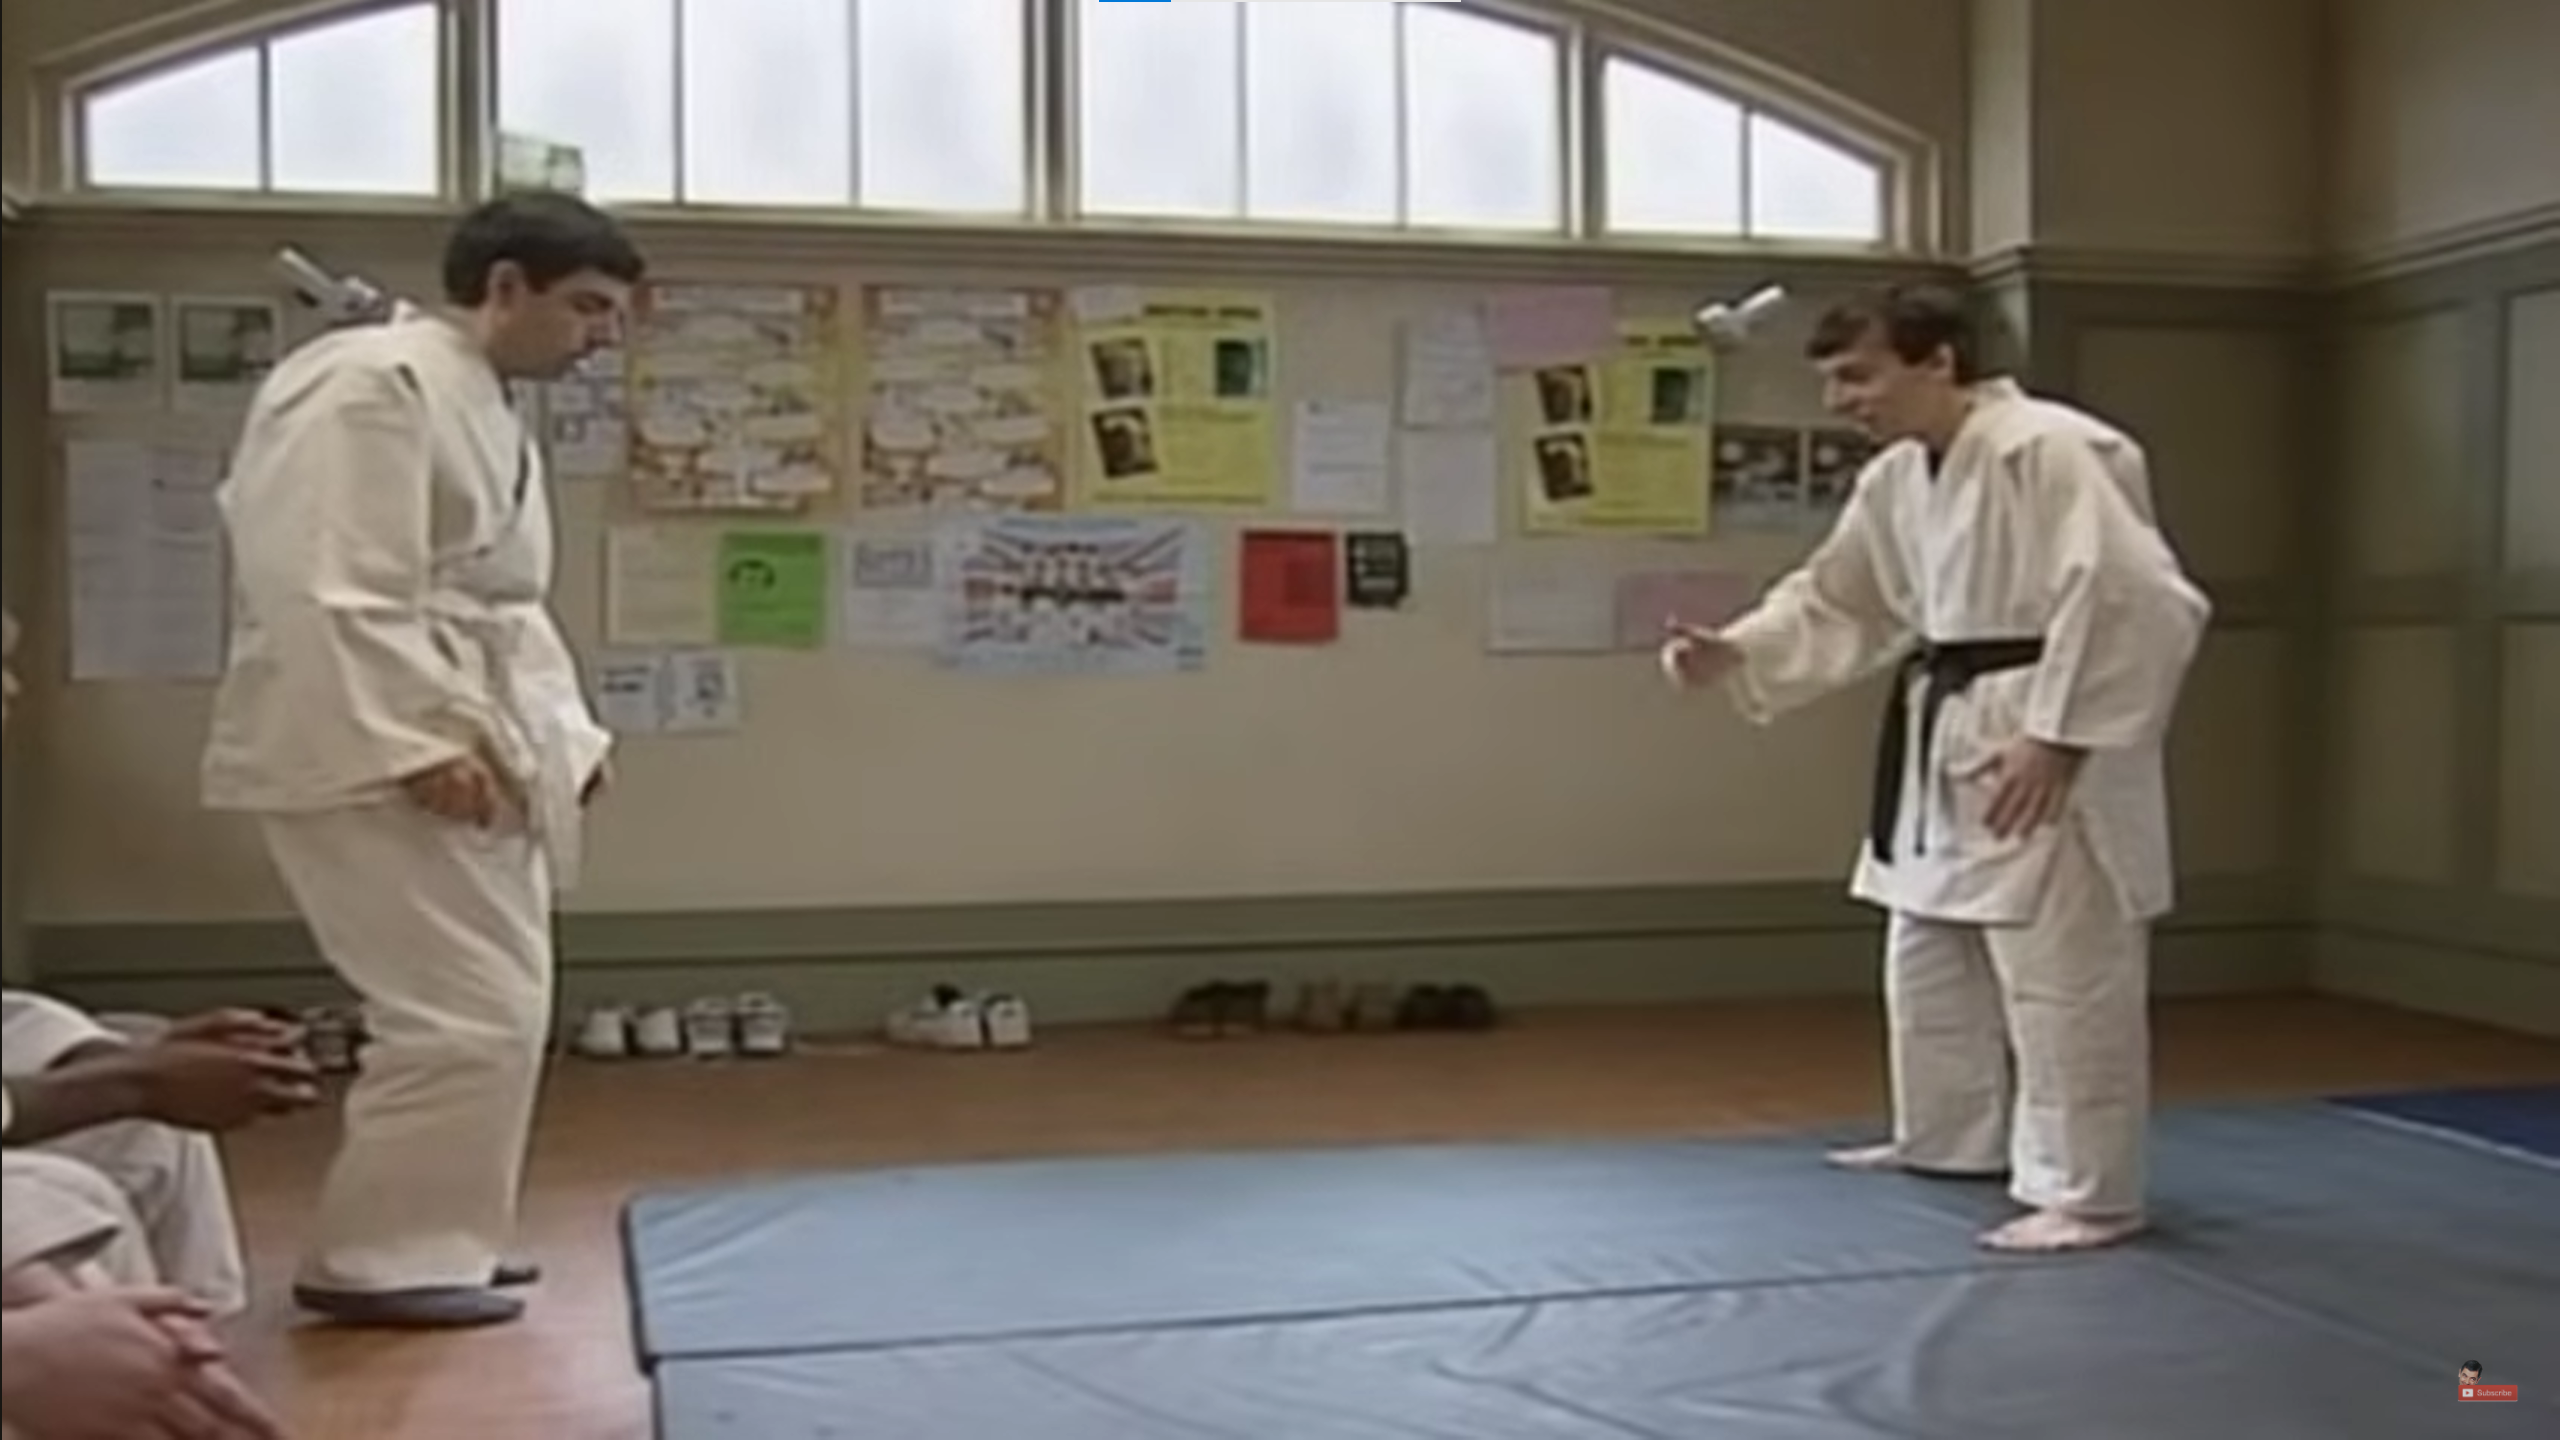
\includegraphics[width=\linewidth]{images/Oblivious.png}
        \end{column}
        
        \begin{column}{0.45\textwidth}
            \textbf{Adaptive Adversary}
            \begin{itemize}
                \item \textbf{Definition:} Adjusts based on algorithm's past actions.
                \item \textbf{Traits:}
                \begin{itemize}
                    \item Responsive and dynamic.
                    \item Harder to counter.
                \end{itemize}
            \end{itemize}
            \vspace{0.2cm}
            
\includegraphics[width=\linewidth]{images/adaptive.jpg}
        \end{column}
    \end{columns}

\end{frame}
\section{Building the Algorithm}
\subsection{Follow the Perturbed Leader (FPL)}
\begin{frame}{Introducing Follow the Perturbed Leader (FPL)}
    \begin{itemize}
        \item \textbf{Overview:}
        \begin{itemize}
            \item FPL is a randomized online algorithm that minimizes regret in adversarial settings by adding noise to each expert's cumulative loss and selecting the leader with the lowest perturbed loss.
        \end{itemize}
        \item \textbf{Algorithm Steps:}
            \begin{enumerate}
                \item \textbf{Initialization:} Set cumulative loss \( L_i(0) = 0 \) for all experts \( i \).
                \item \textbf{For each round } \( t = 1, 2, \ldots, T \):
                    \begin{enumerate}
                        \item \textbf{Perturbation:} Draw a random perturbation \( \gamma_i \) for each expert \( i \) from a specified distribution (e.g., exponential).
                        \item \textbf{Leader Selection:} Choose the expert \( i^* \) with the minimum \( L_i(t-1) + \gamma_i \).
                        \item \textbf{Decision:} Follow the prediction of expert \( i^* \).
                        \item \textbf{Update:} Update the cumulative loss \( L_i(t) = L_i(t-1) + \ell_i(t) \) for each expert.
                    \end{enumerate}
            \end{enumerate}
    \end{itemize}
\end{frame}

\begin{frame}{Why Perturbation?}
    \begin{table}[ht]
        \centering
        \caption{Daily Weather Predictions, Outcomes, and Probability of Mistake using Random Weighted Majority}
        \begin{tabular}{|c|c|c|c|c|}
            \hline
            \textbf{Day} & \textbf{Father} & \textbf{Mother} & \textbf{$\mathbf{P}$ of Mistake} & \textbf{Actual Weather} \\
            \hline
            1 & \texttt{Rain} & \texttt{No Rain} & $\frac{1}{2}$ & \texttt{Rain} \\
            \hline
            2 & \texttt{Rain} & \texttt{No Rain} & $\frac{1}{2}$  & \texttt{No Rain} \\
            \hline
            3 & \texttt{Rain} & \texttt{No Rain} & $\frac{1}{2}$  & \texttt{Rain} \\
            \hline
            4 & \texttt{Rain} & \texttt{No Rain} & $\frac{1}{2}$  & \texttt{No Rain} \\
            \hline
            5 & \texttt{Rain} & \texttt{No Rain} & $\frac{1}{2}$  & \texttt{Rain} \\
            \hline
        \end{tabular}
    \end{table}
\end{frame}

\begin{frame}{Regret Bound for GEX}
    \textbf{Lemma:}
    Let $S \subseteq \mathbb{R}^n$ be a set of (not necessarily positive) decisions, and 
    $k^t = [\mathbf{c}^1, \ldots, \mathbf{c}^T]$ a set of cost vectors on those decisions, such that 
    $\lvert \mathbf{c}^t \cdot \mathbf{x} \rvert \leq R$ for all $\mathbf{x} \in S$ and $\mathbf{c}^t \in k^t$. 
    Then, there is an algorithm $\mathcal{A}(\varepsilon)$ that achieves
    \begin{align*}
        E[\text{loss}(\mathcal{A}(\varepsilon), k^t)] \leq \text{OPT}(k^t) + \varepsilon (4n + 2) R^2 T + \frac{4n}{\varepsilon}
    \end{align*}
\end{frame}

\subsection{Connecting Oblivious and Adaptive Adversaries}
\begin{frame}{Use your Maximum Power}
    In general, oblivious adversaries are easier to handle than adaptive adversaries. However, we can convert an oblivious adversary to an adaptive by being pessimistic.
    \begin{figure}
        \centering
        
\includegraphics[width=0.4\linewidth]{images/An evil adversary in machine learning using its maximum power, with a focus on machine learning and optimization.png}
        \caption{An evil adversary in machine learning using its maximum power}
    \end{figure}
\end{frame}

\begin{frame}{Regret Bound for Any Adversary}
    \textbf{Lemma:}
        Fix $T$, let $H^*$ be the set of decision histories of length $0$ to $T-1$, and let $K^*$ be the set of all cost histories of length $0$ to $T-1$. Then, fix a decision algorithm $\mathcal{A} : K^* \to \Delta(S)$, where $\Delta(S)$ is the set of probability distributions on the set $S$ of possible decisions. Define
        \begin{align*}
            R(\mathcal{A}, \mathcal{V}) = \mathbb{E}_{\mathcal{A}, \mathcal{V}} \left[ \sum_{t=1}^T \mathbf{c}^t \cdot \mathbf{x}^t - \min_{\mathbf{x} \in S} \sum_{t=1}^T \mathbf{c}^t \cdot \mathbf{x} \right].
        \end{align*}
        Let $\mathcal{V}$ be an arbitrary adversary. Then, there exists an oblivious adversary $\mathcal{V}'$ such that
        \begin{align*}            
            R(\mathcal{A}, \mathcal{V}') \geq R(\mathcal{A}, \mathcal{V}).
        \end{align*}
\end{frame}
\subsection{Connection to Bandit Algorithms}
\begin{frame}{Exploration and Exploitation}
    Now that we have a way to convert an oblivious adversary to an adaptive one, we can focus on using online optimization algorithms to solve bandit problems.
    \begin{itemize}
        \item \textbf{Exploration:} Use the perturbation or other methods to explore different experts and their predictions.
        \item \textbf{Exploitation:} Follow the leader to exploit the best-performing expert.
    \end{itemize}
    \begin{figure}
        \centering
        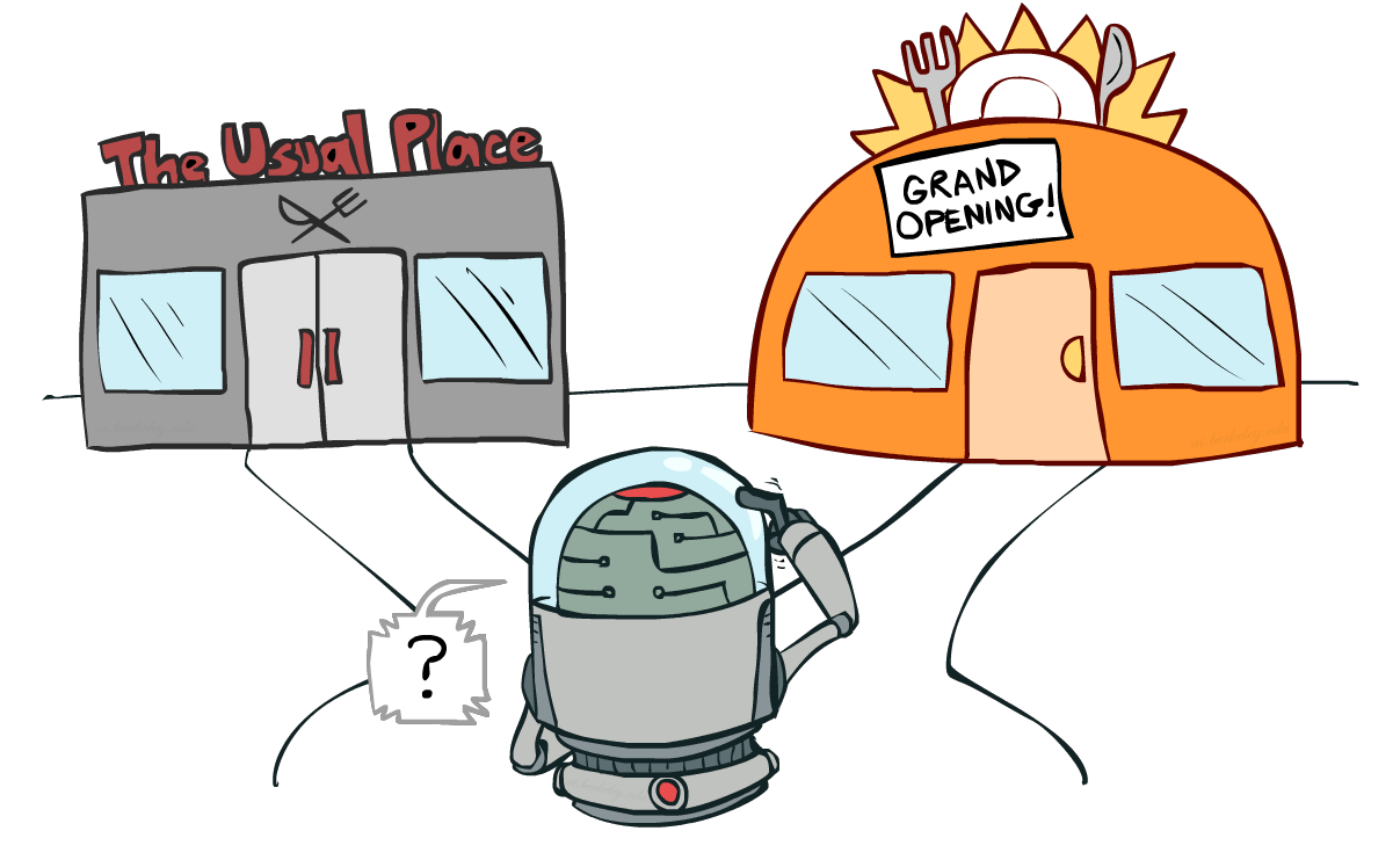
\includegraphics[width=0.5\linewidth]{images/exploration_vs_exploitation.png}
        \caption{Exploration vs. Exploitation in Bandit Algorithms}
    \end{figure}
\end{frame}

\subsection{How to Explore Bounded Infinite Sets}
\begin{frame}{Usage of Basis}
    \begin{itemize}
        \item \textbf{Definition:} A basis $B = \{\mathbf{b}_1, \ldots, \mathbf{b}_n\}$ is a set of linearly independent vectors that span a vector space.
        \item \textbf{Advantages:}
        \begin{itemize}
            \item Reduces the problem of exploring an infinite set to exploring a finite set.
            \item Simplifies the decision-making process.
        \end{itemize}
        \item \textbf{Dimention:} At most $n$.
    \end{itemize}
\end{frame}

\section{BGA Algorithm}
\subsection{Problem Formulation}
\begin{frame}{Problem Formulation}
    \scriptsize
    \begin{table}[H]
        \centering
        \caption{Summary of notation}
        \begin{tabular}{ll}
        \hline
        $S \subseteq \mathbb{R}^n$ & set of decisions, a compact subset of $\mathbb{R}^n$ \\
        $D \in \mathbb{R}$ & $L_1$ bound on diameter of $S$, $\forall \mathbf{x}, \mathbf{y} \in S$, $\lvert \mathbf{x} - \mathbf{y} \rvert_1 \leq D$ \\
        $n \in \mathbb{N}$ & dimension of decision space \\
        $\mathcal{V} : H^* \to \mathbb{R}^n$ & adversary, function from decision histories to cost vectors \\
        $\mathcal{A}$ & an online optimization algorithm \\
        $\mathbf{c}^t \in \mathbb{R}^n$ & cost vector on time $t$ \\
        $\hat{\mathbf{c}}^t \in \mathbb{R}^n$ & BGA's estimate of the cost vector on time $t$ \\
        $M \in \mathbb{R}^+$ & bound on single-iteration cost, $\lvert \mathbf{c}^t \cdot \mathbf{x}^t \rvert \leq M$ \\
        $B \subseteq S$ & sampling basis $B = \{\mathbf{b}_1, \ldots, \mathbf{b}_n\}$ \\
        $\ell^t \in [-M, M]^n$ & vector, $\ell^t_i = \mathbf{c}^t \cdot \mathbf{b}_i$ for $\mathbf{b}_i \in B$ \\
        $\hat{\ell}^t \in \mathbb{R}^n$ & BGA's estimate of $\ell^t$ \\
        $T \in \mathbb{N}$ & end of time, index of final iteration \\
        $\mathbf{x}^t \in S$ & BGA's decision on time $t$ \\
        $\tilde{\mathbf{x}}^t \in S$ & decision recommended by GEX on time $t$ \\
        $\chi^t \in \{0, 1\}$ & indicator, $\chi^t = 1$ if BGA explores on $t$, $0$ otherwise \\
        $\gamma \in [0, 1]$ & the probability BGA explores on each timestep \\
        $\tilde{z}^t \in [-R, R]$ & loss of GEX, $\tilde{z}^t = \hat{\mathbf{c}}^t \cdot \tilde{\mathbf{x}}^t$ \\
        \hline
        \end{tabular}
        \end{table}
\end{frame}
\begin{frame}{Bandit-style Geometric decision algorithm against an Adaptive adversary}
    \begin{algorithm}[H]
        \scriptsize
        \caption{BGA}
        \begin{algorithmic}[1]
        \State \textbf{Choose parameters} $\gamma$ and $\epsilon$, \textbf{where} $\epsilon$ \textbf{is a parameter of GEX}
        \State $t = 1$
        \State \textbf{Fix a basis} $B = \{\mathbf{b}_1, \ldots, \mathbf{b}_n\} \subseteq S$
        \While{playing}
            \State \textbf{Let} $\chi^t = 1$ \textbf{with probability} $\gamma$ \textbf{and} $\chi^t = 0$ \textbf{otherwise}
            \If{$\chi^t = 0$}
                \State \textbf{Select} $\mathbf{x}^t$ \textbf{from the distribution} $\text{GEX}(\hat{\mathbf{c}}^1, \ldots, \hat{\mathbf{c}}^{t-1})$
                \State \textbf{Incur cost} $z^t = \mathbf{c}^t \cdot \mathbf{x}^t$
                \State $\hat{\mathbf{c}}^t = 0 \in \mathbb{R}^n$
            \Else
                \State \textbf{Draw} $j$ \textbf{uniformly at random from} $\{1, \ldots, n\}$
                \State $\mathbf{x}^t = \mathbf{b}_j$
                \State \textbf{Incur cost and observe} $z^t = \mathbf{c}^t \cdot \mathbf{x}^t$
                \State \textbf{Define} $\hat{\ell}^t$ \textbf{by} $\hat{\ell}^t_i = 0$ \textbf{for} $i \neq j$ \textbf{and} $\hat{\ell}^t_j = (n / \gamma) z^t$
                \State $\hat{\mathbf{c}}^t = (B^\top)^{-1} \hat{\ell}^t$
            \EndIf
            \State $\hat{\mathbf{c}}^{1:t} = \hat{\mathbf{c}}^{1:t-1} + \hat{\mathbf{c}}^t$
            \State $t = t + 1$
        \EndWhile
        \end{algorithmic}
        \end{algorithm}
\end{frame}        
\subsection{How BGA Works}

\begin{frame}{How BGA Works - Part 1}
    \scriptsize % Optional: Reduce font size to fit content

    \begin{itemize}
        \item \textbf{Initialization:}
        \begin{itemize}
            \item Choose parameters $\gamma$ and $\epsilon$, where $\epsilon$ is a parameter of GEX.
            \item Set $t \gets 1$.
            \item Fix a basis $B = \{\mathbf{b}_1, \ldots, \mathbf{b}_n\} \subseteq S$.
        \end{itemize}
        \pause

        \item \textbf{Main Loop:} \textbf{While} playing \textbf{do}
        \begin{itemize}
            \item Let $\chi^t = 1$ with probability $\gamma$ and $\chi^t = 0$ otherwise.
            \pause

            \item \textbf{If} $\chi^t = 0$ \textbf{then}
            \begin{itemize}
                \item Select $\mathbf{x}^t$ from the distribution $\text{GEX}(\hat{\mathbf{c}}^1, \ldots, \hat{\mathbf{c}}^{t-1})$.
                \item Incur cost $z^t = \mathbf{c}^t \cdot \mathbf{x}^t$.
                \item Set $\hat{\mathbf{c}}^t = \mathbf{0} \in \mathbb{R}^n$.
            \end{itemize}
        \end{itemize}
    \end{itemize}
\end{frame}

\begin{frame}{How BGA Works - Part 2}
    \begin{itemize}
        \item \textbf{Else}
        \begin{itemize}
            \item Draw $j$ uniformly at random from $\{1, \ldots, n\}$.
            \item Set $\mathbf{x}^t = \mathbf{b}_j$.
            \item Incur cost and observe $z^t = \mathbf{c}^t \cdot \mathbf{x}^t$.
            \item Define $\hat{\ell}^t$ by:
            \begin{itemize}
                \item $\hat{\ell}^t_i = 0$ for all $i \neq j$.
                \item $\hat{\ell}^t_j = \left(\dfrac{n}{\gamma}\right) z^t$.
            \end{itemize}
            \item Set $\hat{\mathbf{c}}^t = (B^\top)^{-1} \hat{\ell}^t$.
        \end{itemize}
        \pause

        \item Update cumulative costs:
        \begin{itemize}
            \item $\hat{\mathbf{c}}^{1:t} = \hat{\mathbf{c}}^{1:t-1} + \hat{\mathbf{c}}^t$.
            \item Increment time step: $t \gets t + 1$.
        \end{itemize}
    \end{itemize}
\end{frame}

\subsection{Regret Bound for BGA}
\begin{frame}{Regret Bound for BGA}
    The regret of the BGA algorithm is bounded by
    \begin{align*}
        E[\text{loss}(\text{BGA})] \leq (1 - \gamma) E[\text{loss}(\text{GEX})] + \gamma MT
    \end{align*}
    \texttt{Intuition:} BGA explores with probability $\gamma$ and exploits with probability $1 - \gamma$. \\
    \textbf{Order of Regret:} It can be shown that the regret of BGA is of order $O(T^{3/4}\sqrt{ln T})$.
\end{frame}
\section{Future Work}
\begin{frame}{Future Work}
    \begin{enumerate}
        \item \textbf{Exploring while Exploiting:} I think the exploitation phase has some information that can be used to explore better.
        \item \textbf{Hyperparameter Tuning:} The parameters $\gamma$ can be tuned to improve the performance of the algorithm.
        \item \textbf{Game Theory:} The algorithm can be viewed as an Stackelberg game. Thus there is a possibility of using game theory.
        \item \textbf{Experiments:} The algorithm hasn't tested on real-world data. It would be interesting to see how it performs in practice.
        \item \textbf{Bound Tightening:} Investigate whether the current bounds of \( O(T^{3/4} \sqrt{\ln T}) \) against adaptive adversaries and \( O(T^{2/3}) \) against oblivious adversaries can be improved to \( O(\sqrt{T}) \).
        \end{enumerate}
\end{frame}
\begin{frame}[allowframebreaks]{References}
    \begin{thebibliography}{10}

        \beamertemplatebookbibitems
        % Books
        \bibitem{lattimore2020bandit}
        Tor Lattimore and Csaba Szepesv{\'a}ri.
        \newblock \emph{Bandit Algorithms}.
        \newblock Cambridge University Press, 2020.

        \bibitem{hazan2016online}
        Elad Hazan.
        \newblock \emph{Introduction to Online Convex Optimization}.
        \newblock Cambridge University Press, 2016.

        \beamertemplatearticlebibitems
        % Articles
        \bibitem{mcmahan2004online}
        H.~B. McMahan and A.~Blum.
        \newblock \emph{Online Geometric Optimization in the Bandit Setting Against an Adaptive Adversary}.
        \newblock In J.~Shawe-Taylor and Y.~Singer, editors, \emph{Learning Theory}, Springer Berlin Heidelberg, 2004, pp. 109--123.

        \bibitem{auer2002nonstochastic}
        P.~Auer, N.~Cesa-Bianchi, Y.~Freund, and R.~E.~Schapire.
        \newblock \emph{The Nonstochastic Multiarmed Bandit Problem}.
        \newblock \emph{SIAM Journal on Computing}, 32(1):48--77, 2002.

        \bibitem{kalai2005efficient}
        A.~Kalai and S.~Vempala.
        \newblock \emph{Efficient algorithms for online decision problems}.
        \newblock \emph{Journal of Computer and System Sciences}, 71(3):291--307, 2005.
    \end{thebibliography}
\end{frame}

\end{document}
